\documentclass{beamer}
\mode<presentation>
\usepackage{amsmath}
\usepackage{amssymb}
\usepackage{algorithmic}
%\usepackage{advdate}
\usepackage{adjustbox}
\usepackage{subcaption}
\usepackage{enumitem}
\usepackage{multicol}
\usepackage{mathtools}
\usepackage{listings}
\usepackage{url}
\def\UrlBreaks{\do\/\do-}
\usetheme{Boadilla}
\usecolortheme{lily}
\setbeamertemplate{footline}
{
	\leavevmode%
	\hbox{%
		\begin{beamercolorbox}[wd=\paperwidth,ht=2.25ex,dp=1ex,right]{author in head/foot}%
			\insertframenumber{} / \inserttotalframenumber\hspace*{2ex} 
	\end{beamercolorbox}}%
	\vskip0pt%
}
\setbeamertemplate{navigation symbols}{}

\providecommand{\nCr}[2]{\,^{#1}C_{#2}} % nCr
\providecommand{\nPr}[2]{\,^{#1}P_{#2}} % nPr
\providecommand{\mbf}{\mathbf}
\providecommand{\pr}[1]{\ensuremath{\Pr\left(#1\right)}}
\providecommand{\qfunc}[1]{\ensuremath{Q\left(#1\right)}}
\providecommand{\sbrak}[1]{\ensuremath{{}\left[#1\right]}}
\providecommand{\lsbrak}[1]{\ensuremath{{}\left[#1\right.}}
\providecommand{\rsbrak}[1]{\ensuremath{{}\left.#1\right]}}
\providecommand{\brak}[1]{\ensuremath{\left(#1\right)}}
\providecommand{\lbrak}[1]{\ensuremath{\left(#1\right.}}
\providecommand{\rbrak}[1]{\ensuremath{\left.#1\right)}}
\providecommand{\cbrak}[1]{\ensuremath{\left\{#1\right\}}}
\providecommand{\lcbrak}[1]{\ensuremath{\left\{#1\right.}}
\providecommand{\rcbrak}[1]{\ensuremath{\left.#1\right\}}}
\theoremstyle{remark}
\newtheorem{rem}{Remark}
\newcommand{\sgn}{\mathop{\mathrm{sgn}}}
\providecommand{\abs}[1]{\left\vert#1\right\vert}
\providecommand{\res}[1]{\Res\displaylimits_{#1}} 
\providecommand{\norm}[1]{\lVert#1\rVert}
\providecommand{\mtx}[1]{\mathbf{#1}}
\providecommand{\mean}[1]{E\left[ #1 \right]}
\providecommand{\fourier}{\overset{\mathcal{F}}{ \rightleftharpoons}}
%\providecommand{\hilbert}{\overset{\mathcal{H}}{ \rightleftharpoons}}
\providecommand{\system}{\overset{\mathcal{H}}{ \longleftrightarrow}}
%\newcommand{\solution}[2]{\textbf{Solution:}{#1}}
%\newcommand{\solution}{\noindent \textbf{Solution: }}
\providecommand{\dec}[2]{\ensuremath{\overset{#1}{\underset{#2}{\gtrless}}}}
\newcommand{\myvec}[1]{\ensuremath{\begin{pmatrix}#1\end{pmatrix}}}
\let\vec\mathbf

\lstset{
	%language=C,
	frame=single, 
	% breaklines=true,
	columns=fullflexible
}

\numberwithin{equation}{section}

\title{Identify and Solve the Linear Equations}
\author{Eshan Sharma - EE24BTECH11022}

\date{\today} 
\begin{document}
	
	\begin{frame}
		\titlepage
	\end{frame}
	
	\section*{Outline}
	\begin{frame}
		\tableofcontents
	\end{frame}
	
	\section{Problem}
	\begin{frame}
		\frametitle{Problem Statement}
		Meena went to a bank to withdraw 2000. She asked the cashier to give her 50 and 100 notes only. Meena got 25 notes in all. Find how many notes of 50 and 100 she received.
	\end{frame}
	
	%\subsection{Literature}
	\section{Solution}
	
	\subsection{Linear Equations}
	\begin{frame}
		\frametitle{Linear Equations}
		Let the number of 50 notes be \(x\) and the number of 100 notes be \(y\). From the problem, we form the following equations:
		\begin{align}
			x + y &= 25 \quad \text{(1)} \\
			50x + 100y &= 2000 \quad \text{(2)}
		\end{align}
		
		The system of equations can be written as:
		\[
		A \mathbf{x} = \mathbf{b}
		\]
		where
		\[
		A = \begin{pmatrix} 1 & 1 \\ 50 & 100 \end{pmatrix}, \quad \mathbf{x} = \begin{pmatrix} x \\ y \end{pmatrix}, \quad \mathbf{b} = \begin{pmatrix} 25 \\ 2000 \end{pmatrix}.
		\]
	\end{frame}
	
	\subsection{LU Decomposition}
	\begin{frame}[allowframebreaks]
		\frametitle{LU Decomposition}
		The LU decomposition splits \(A\) into a lower triangular matrix \(L\) and an upper triangular matrix \(U\) such that:
		\[
		A = LU
		\]
		where:
		\[
		L = \begin{pmatrix} 1 & 0 & 0 & \cdots & 0 \\ l_{21} & 1 & 0 & \cdots & 0 \\ l_{31} & l_{32} & 1 & \cdots & 0 \\ \vdots & \vdots & \vdots & \ddots & 0 \\ l_{n1} & l_{n2} & l_{n3} & \cdots & 1 \end{pmatrix}, \quad
		U = \begin{pmatrix} u_{11} & u_{12} & u_{13} & \cdots & u_{1n} \\ 0 & u_{22} & u_{23} & \cdots & u_{2n} \\ 0 & 0 & u_{33} & \cdots & u_{3n} \\ \vdots & \vdots & \vdots & \ddots & u_{n-1,n} \\ 0 & 0 & 0 & \cdots & u_{nn} \end{pmatrix}.
		\]
		
		The Doolittle algorithm is computed as follows:
		
		1. For \(U\):
		\[
		u_{ij} = a_{ij} - \sum_{k=1}^{i-1} l_{ik} u_{kj}, \quad \text{for } i \leq j.
		\]
		
		2. For \(L\):
		\[
		l_{ij} = \frac{1}{u_{ii}} \left(a_{ij} - \sum_{k=1}^{i-1} l_{ik} u_{kj} \right), \quad \text{for } i > j.
		\]
		
		3. Diagonal entries of \(L\) are set to 1:
		\[
		l_{ii} = 1, \quad \text{for all } i.
		\]
		
		Using these general formulas, we compute \(L\) and \(U\) for our specific problem:
		\[
		A = \begin{pmatrix} 1 & 1 \\ 50 & 100 \end{pmatrix}.
		\]
		\textbf{Step 3.1: Compute the elements of \(L\) and \(U\)}\\
		\begin{align}
			u_{11} &= a_{11} = 1, \quad u_{12} = a_{12} = 1 \\
			l_{21} &= \frac{a_{21}}{u_{11}} = \frac{50}{1} = 50 \\
			u_{22} &= a_{22} - l_{21}u_{12} = 100 - 50 \cdot 1 = 50
		\end{align}
		
		Thus, the matrices \(L\) and \(U\) are:
		\[
		L = \begin{pmatrix} 1 & 0 \\ 50 & 1 \end{pmatrix}, \quad U = \begin{pmatrix} 1 & 1 \\ 0 & 50 \end{pmatrix}.
		\]
		
	\end{frame}

	
	\subsection{Forward and Backward Substitution}
	\begin{frame}[allowframebreaks]
		\frametitle{Forward and Backward Substitution}
		First, solve \(L \mathbf{y} = \mathbf{b}\) for \(\mathbf{y}\):
		\[
		\begin{pmatrix} 1 & 0 \\ 50 & 1 \end{pmatrix} \begin{pmatrix} y_1 \\ y_2 \end{pmatrix} = \begin{pmatrix} 25 \\ 2000 \end{pmatrix}.
		\]
		This gives:
		\begin{align}
			y_1 &= 25, \\
			50y_1 + y_2 &= 2000 \quad \Rightarrow \quad 50(25) + y_2 = 2000 \quad \Rightarrow \quad y_2 = 750.
		\end{align}
		Thus, \(\mathbf{y} = \begin{pmatrix} 25 \\ 750 \end{pmatrix}\).
		
		Next, solve \(U \mathbf{x} = \mathbf{y}\) for \(\mathbf{x}\):
		\[
		\begin{pmatrix} 1 & 1 \\ 0 & 50 \end{pmatrix} \begin{pmatrix} x \\ y \end{pmatrix} = \begin{pmatrix} 25 \\ 750 \end{pmatrix}.
		\]
		This gives:
		\begin{align}
			50y &= 750 \quad \Rightarrow \quad y = 15, \\
			x + y &= 25 \quad \Rightarrow \quad x + 15 = 25 \quad \Rightarrow \quad x = 10.
		\end{align}
		
		The number of 50 notes is \(x = 10\), and the number of 100 notes is \(y = 15\).
	\end{frame}
	
	
	\subsection{Plotting the curve}
	\begin{frame}
		\frametitle{Plotting the curve}
		\begin{figure}[h]
			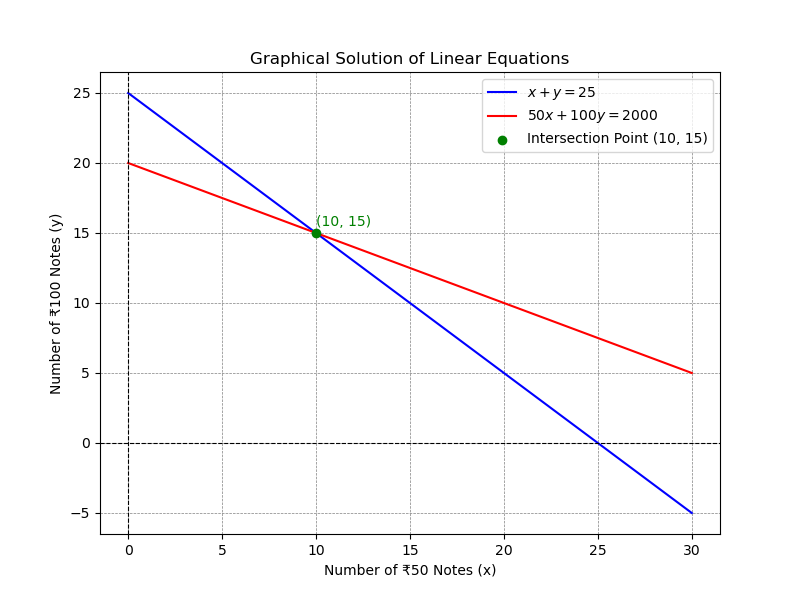
\includegraphics[scale=0.5]{fig.png}
			\centering
		\end{figure}
	\end{frame}

\end{document}